% Suggested LaTeX style template for Masters project report submitted at the
% Department of Computer Science and Technology
%
% Markus Kuhn, May 2022
% (borrowing elements from an earlier template by Steven Hand)

\documentclass[12pt,a4paper,twoside]{report}
% append option ",openright" after "twoside" if you prefer each chapter
% to start on a recto (odd-numbered) page in a double-sided printout

\usepackage[pdfborder={0 0 0}]{hyperref}  % turns references into hyperlinks
\usepackage[vmargin=20mm,hmargin=25mm]{geometry}  % adjust page margins
\usepackage{graphicx} % allows inclusion of PDF, PNG and JPG images
\usepackage{parskip}  % separate paragraphs with vertical space
                      % instead of indenting their first line
\usepackage{setspace} % for \onehalfspacing
\usepackage{refcount} % for counting pages
\usepackage{upquote}  % for correct quotation marks in verbatim text

\usepackage{courier}                  % better listings font
\usepackage{dirtytalk}                % quotations
\usepackage[square,numbers]{natbib}   % citations
\usepackage[chapter]{minted}          % code listings
\usepackage{multirow}                 % multi-row cells in tables
\usepackage{makecell}                 % multi-line cells in tables
\usepackage[subpreambles]{standalone} % tex files as diagrams

\setminted{fontsize=\footnotesize,frame=lines,stripnl=false}

\newif\ifsubmission % Boolean flag for distinguishing submitted/final version

% Change the following lines to your own project title, name, college, course
\title{Void Processes: Minimising privilege by default}
\author{Jake Hillion}
\date{June 2022}
\newcommand{\candidatenumber}{2492A}
\newcommand{\college}{Queens' College}
\newcommand{\course}{Computer Science Tripos, Part III}

% Select which version this is:
% For the (anonymous) submission (without your name or acknowledgements)
% uncomment the following line (or let the makefile do this for you)
\submissiontrue
% For the final version (with your name) leave the above commented.

\begin{document}
%TC:ignore               % don't start counting words yet

\begin{sffamily} % use a sans-serif font for the pro-forma cover sheet

\begin{titlepage}
\makeatletter

% University logo with shield hanging in left margin
\hspace*{-14mm}
\includegraphics[width=65mm]{logo-dcst-colour}

\ifsubmission

% submission proforma cover page for blind marking
\begin{Large}
\vspace{20mm}
Research project report title page

\vspace{35mm}
Candidate \candidatenumber

\vspace{42mm}
\textsl{``\@title''}

\end{Large}

\else

% regular cover page
\begin{center}
\Huge
\vspace{\fill}

\@title
\vspace{\fill}

\@author
\vspace{10mm}

\Large
\college
\vspace{\fill}

\@date
\vspace{\fill}

\end{center}

\fi

\vspace{\fill}
\begin{center}
Submitted in partial fulfillment of the requirements for the\\
\course
\end{center}

\makeatother
\end{titlepage}

\newpage

Total page count: \pageref{lastpage}

% calculate number of pages from
% \label{firstcontentpage} to \label{lastcontentpage} inclusive
\makeatletter
\@tempcnta=\getpagerefnumber{lastcontentpage}\relax%
\advance\@tempcnta by -\getpagerefnumber{firstcontentpage}%
\advance\@tempcnta by 1%
\xdef\contentpages{\the\@tempcnta}%
\makeatother

Main chapters (excluding front-matter, references and appendix):
\contentpages~pages
(pp~\pageref{firstcontentpage}--\pageref{lastcontentpage})

Main chapters word count: 11998

Methodology used to generate that word count:

\begin{quote}
\begin{verbatim}
£ texcount report.tex | grep Words
Words in text: 11023
Words in headers: 108
Words outside text (captions, etc.): 867
\end{verbatim}

\texttt{texcount} macros are used to ensure counting begins on the first content page and ends on the last content page.
\end{quote}

\end{sffamily}

\onehalfspacing

\ifsubmission\else
% not included in submission for blind marking:

\newpage
{\Huge \bf Declaration}

\vspace{24pt}

I, Jake Hillion of Queens' College, being a candidate for Computer
Science Tripos, Part III, hereby declare that this report and the
work described in it are my own work, unaided except as may be
specified below, and that the report does not contain material that
has already been used to any substantial extent for a comparable
purpose.

\vspace{60pt}
\textbf{Signed}:  Jake Hillion

\vspace{12pt}
\textbf{Date}: \today


\vfill

This dissertation is copyright \copyright 2022 Jake Hillion. 
\\
All trademarks used in this dissertation are hereby acknowledged.

\fi
\cleardoublepage % preserve page numbers after missing declaration

\chapter*{Abstract}

Void processes intend to make it easier for all developers to produce effectively privilege separated applications. The project has two primary goals: show the merits of starting from zero privilege, and provide the utilities to make this feasible for the average developer.

Building void processes involves first reliably removing all privilege from a process then systematically adding back in what is required, and no more. This project utilises namespaces on Linux to revoke privilege from an application, showing how this can be done and why its easier in some domains than others. We then show how to inject sufficient privilege for applications to perform useful work, developing new APIs that are friendly for privilege separation. These elements compose a shim called the void orchestrator, a framework for restricting Linux processes.

Two example applications are presented to demonstrate the utility of a shim helping with privilege separation. The startup performance is negatively affected by the design of the kernel, and future work is proposed to aid this. After the delay in startup, applications developed within this framework are shown to be highly performant.

Computer Scientists need better tools to handle the continuing prevalence of vulnerabilities in computer software. Starting from nothing is a new approach to privilege separation on Linux that has noticeable benefits. Linux should focus on reducing namespace creation latency however they can, and beginning from nothing is a good way to achieve that.

\cleardoublepage % preserve page numbers after missing acknowledgements

\setcounter{tocdepth}{1} % only show up to sections in the table of contents
\tableofcontents
%\listoffigures
%\listoftables
%\lstlistoflistings

%TC:endignore            % start word count here
\chapter{Introduction}
\label{firstcontentpage} % start page count here
\label{chap:introduction}

Newly spawned processes on modern Linux are exposed to a myriad of attack vectors and unnecessary privilege: whether the hundreds of system calls available, \texttt{procfs}, exposure of filesystem objects, or the ability to connect to arbitrary hosts on the Internet.

This thesis argues that we need a framework to restrict Linux processes - removing access to ambient resources by default - and provide APIs to minimally unlock application access to the outside world. This approach would have saved many existing applications from remote exploits by ensuring that processes which handle sensitive user data are sufficiently deprivileged to utilise remote code execution. The resulting programming interfaces are far easier to reason about for a novice programmer, and encourage proactive consideration of security rather than reactive when flaws are exposed.

This project presents a system, the void orchestrator, to enable application developers to build upwards from a point of zero-privilege. I give a summary of the privilege separation techniques currently employed in production (§\ref{chap:priv-sep}) and details on how to create an empty set of namespaces to remove all privilege in Linux (§\ref{chap:entering-the-void}). The shortcomings of Linux when creating empty namespaces are discussed (§\ref{sec:voiding-mount},§\ref{sec:voiding-user},§\ref{sec:voiding-cgroup}), before setting forth the methods for re-adding features in each of these domains (§\ref{chap:filling-the-void}). Finally, two example applications are built and evaluated (§\ref{chap:building-apps}) to show the utility of the system. This report aims to demonstrate the value of a paradigm shift from reducing a moving target of privilege to adding only what is necessary.

Prior work exists for privilege separation, including: virtual machines (§\ref{sec:priv-sep-another-machine}); containers (§\ref{sec:priv-sep-perspective}); object capabilities (§\ref{sec:priv-sep-ownership}); unikernels; and applications which run directly on a Linux host, potentially employing privilege separation of their own (§\ref{sec:priv-sep-process}, §\ref{sec:priv-sep-time}). These environments are plotted in Figure \ref{fig:attack-vs-changes}, which compares the environment's support for Linux APIs and the attack surface remaining. Void processes represent a strong compromise between a rich subset of Linux for applications - reducing code changes - and significantly reducing the attack surface (demonstrated in §\ref{chap:entering-the-void}).

\begin{figure}
    \centering
    \includestandalone[width=0.8\textwidth]{diagrams/attack-surface-vs-linux-compatibility}
    
    \caption{Privilege separated environments plotted to compare the number of application changes required against the remaining attack surface of the environment.}
    \label{fig:attack-vs-changes}
\end{figure}


\chapter{Privilege Separation}
\label{chap:priv-sep}

Many attack vectors exist in software, notably in argument processing \citep{the_mitre_corporation_improper_2006} and deserialisation \citep{the_mitre_corporation_deserialization_2006}. Creating secure applications requires one of two things: creating applications without security bugs, or separating the parts of the application with the potential to cause damage from the parts most likely to contain bugs. Though many efforts have been made to create correct applications and protocols \citep{hawblitzel_ironfleet_2015,ma_i4_2019,nelson_scaling_2019}, the use of such technology is far from widespread and security related bugs in applications are still frequent - over 20,000 Common Vulnerability and Exposure (CVE) reports were published in 2021 \footnote{\url{https://www.cve.org/About/Metrics}}. Rather than attempting to avoid bugs, we primarily employ privilege separation: ensuring that the privileged portion of the application is separated from the portion which is likely to be attacked. This chapter details what privilege separation is, why it is useful, and a summary of some of the privilege separation techniques available in modern Unices. Many of these techniques are included in some form in the final design for void processes.

\section{Privilege separation by process}
\label{sec:priv-sep-process}

The basic unit of privilege separation on Unix is a process. If it's possible for an attacker to gain remote code execution in a process, the attacker gains access to all of that process's privilege. Reducing the privilege of a process reduces the value of attacking that process. One solution to reducing privilege per process is to take a previously monolithic application and split it into multiple smaller processes. Consider a TLS supporting web server that must have access to the certificate's private keys and also process user requests. If these elements are split into different processes a compromised user data handling process cannot access the contents of the private keys.

Application design in this paradigm is similar to that of a distributed system, where multiple asynchronous systems must interact over various communication channels. As an application becomes more like a networked system, serialisation and deserialisation become more common. As deserialisation is a very common source of exploits \citep{the_mitre_corporation_deserialization_2006}, this adds the potential for new flaws in the application.

OpenBSD is a UNIX operating system with an emphasis on security. A recent bug in OpenBSD's \texttt{sshd} highlights the utility of privilege separation \citep{the_openbsd_foundation_openssh_2022}. An integer overflow in the pre-authentication logic of the SSH daemon allowed a motivated attacker to exploit incorrect logic paths and gain access without authentication. Privilege separation ensures that the process with this bug, the pre-authentication process, is separated from the process which is able to be exploited, the highly privileged daemon.

In 2003, privilege separation was added to the \texttt{syslogd} daemon of OpenBSD \citep{madhavapeddy_privsepc_2003}. The system consists of a highly privileged parent process and a network accepting child process. The child process can initially make many requests from the parent, but these decrease as the application progresses. This pattern allows for restarting of the service while keeping the section which processed user data strongly separated from the process which remains privileged - the child process can cause its own restart while not holding enough privilege to execute that restart itself. An overview of the data flow is provided in Figure \ref{fig:openbsd-syslogd-privsep}.

\begin{figure}
    \centering
    \includestandalone[width=0.4\textwidth]{diagrams/openbsd-syslogd-privsep}
    
    \caption{Separation of privileged access from untrusted user data in OpenBSD's privilege separated syslogd design compared to the previous. The process which handles untrusted data is separated from the privileged process and uses RPC to communicate.}
    \label{fig:openbsd-syslogd-privsep}
\end{figure}

\section{Privilege separation by time}
\label{sec:priv-sep-time}

Many applications can privilege separate by using a single process which reduces its level of privilege as the application makes progress. One begins with high privilege for opening sensitive resources, such as a listening socket below port 1000. After this has been completed, the ability to do so is dropped. One of the simplest ways to do this is to change user using \texttt{setuid(2)} after the privileged requirements are complete. An API such as OpenBSD's \texttt{pledge(2)} allows only a pre-specified set of system calls after the call to \texttt{pledge(2)}. A final alternative is to drop explicit capabilities on Linux. Each of these solutions irreversibly reduce the privilege of the process, meaning that any attacker who gains control after the privilege has been dropped cannot take advantage of it.

After dropping privilege, it becomes difficult to do things such as reloading the configuration. The application process no longer has the required privilege to restart itself, as if it could gain it back then dropping the privilege would have had no effect. This avoids having to treat the application as a distributed system as there continues to be only a single process to manage, which is often an easier paradigm to work in. The difficulty in implementing privilege dropping is ensuring that you know what privilege you hold, and drop it as soon as it is no longer required.

\section{Privilege separation by ownership}
\label{sec:priv-sep-ownership}

The previous methods shown each suffer from having to know what their initial privilege is in order to correctly deprivilege. Object capabilities are unforgeable tokens of authority to perform a set of actions on an object.

While the methods looked at until now of privilege separation by process and time are widely supported, object capabilities are less common. Capsicum added object capabilities and was included in FreeBSD 10, released in January 2014 \citep{watson_capsicum_2010}. Capability mode removes access to all global namespaces from a process, allowing only operations on capabilities to continue. These capabilities are commonly those opened before the switch to capability mode, but they can also be sent and received (as file descriptors) or converted from a capability with more privilege to a capability with less.

Capabilities provide good explicit visibility of privilege, making dropping all but what is required a simple task. However, their adoption remains limited at this point. They are unavailable in the latest Linux kernel release (5.17) at the time of writing and there are no plans for their adoption.

\section{Privilege separation by machine}
\label{sec:priv-sep-another-machine}

If developing a web application, one might place the PHP backend on one machine and the database server on another. Even if a bad actor achieves remote access to the exposed PHP backend, they can only access the database server over its exposed API on the network, rather than having control of the machine itself. This allows features such as the database's access control to remain working, limiting the potential damage of an attacker controlling the PHP server.

Virtual machines \citep{barham_xen_2003,vmware_inc_understanding_2008} made the separation of privilege by machine more efficient. Rather than requiring two full servers, one could provide both the PHP backend and the database server on a single physical machine but different virtual machines. This better utilised hardware in a time when hardware speed seemed in excess, and provided very strong isolation (presuming one cannot escape the hypervisor). Though the isolation is strong, there are overheads associated with full virtualisation, and a more performant solution was sought.

\section{Privilege separation by perspective}
\label{sec:priv-sep-perspective}

Namespaces control the view of the world that a process sees. Processes remain the primary method of separation, but utilise namespaces to increase the separation between them. The most common use case of namespaces is providing containers, which approximate virtual machines, providing the appearance of running on an isolated system while sharing the same host. When performing privilege separation with containers, one spawns multiple containers to form a distributed system of applications. It is common to see, for example, a web server and the database that backs it deployed as two separate containers. These separate containers interact entirely over the network. As with virtual machines, if a user achieves remote code execution of the database, it does not extend to the web server. This presents an interesting paradigm of small applications which can and often do run on separate physical hosts combining to provide a unified application experience.

\section{Summary}

This work focuses on the application of namespaces to more conventional privilege separation. Working with a shim which orchestrates the process and namespace layout, void applications seek to provide a completely minimal Linux experience to each void process within the application. There is never a need to drop privileges as processes are created with the absolute minimum privilege necessary to perform correctly. In Chapter \ref{chap:entering-the-void} we discuss each namespace's role in Linux and how to create one which is empty, before explaining in Chapter \ref{chap:filling-the-void} how to reinsert just enough Linux for each process in an application to be able to complete useful work. These combine to form an architecture which minimises privilege by default, motivating highly intentional privilege separation.


\chapter{Entering the Void}
\label{chap:entering-the-void}

\begin{table}
    \begin{center}
    \begin{tabular}{lr|lr|lr|l|l}
        \multicolumn{2}{l}{ns} & \multicolumn{2}{l}{date} & \multicolumn{2}{|l|}{kernel ver.} & ns CVEs & prot. CVEs \\ \hline

        \texttt{mount} & (§\ref{sec:voiding-mount})
            & Feb 2001 & \citep{viro_patchcft_2001}
            & 2.5.2 & \citep{torvalds_linux_2002}
            & 2020-29373
            & \makecell[tl]{2021-23021 \\ 2021-45083 \\ 2022-23653 \vspace{3mm}} \\

        \texttt{ipc} & (§\ref{sec:voiding-ipc})
            & Oct 2006 & \citep{korotaev_patch_2006}
            & 2.6.19 & \citep{linux_kernel_newbies_editors_linux_2006}
            &
            & \makecell[tl]{2015-7613 \vspace{3mm}} \\

        \texttt{uts} & (§\ref{sec:voiding-uts})
            & Oct 2006 & \citep{hallyn_patch_2006}
            & 2.6.19 & \citep{linux_kernel_newbies_editors_linux_2006}
            &
            & \makecell[tl]{\vspace{3mm}} \\

        \texttt{user} & (§\ref{sec:voiding-user})
            & Jul 2007 & \citep{le_goater_user_2007}
            & 2.6.23 & \citep{linux_kernel_newbies_editors_linux_2007}
            & 2021-21284
            & \makecell[tl]{2021-43816 \vspace{3mm}} \\

        \texttt{network} & (§\ref{sec:voiding-net})
            & Oct 2007 & \citep{biederman_net_2007}
            & 2.6.24 & \citep{linux_kernel_newbies_editors_linux_2008}
            & 2009-1360
            & \makecell[tl]{2021-44228 \vspace{3mm}} \\

        \texttt{pid} & (§\ref{sec:voiding-pid})
            & Oct 2006 & \citep{bhattiprolu_patch_2006}
            & 2.6.24 & \citep{linux_kernel_newbies_editors_linux_2008}
            & 2019-20794
            & \makecell[tl]{2012-0056 \vspace{3mm}} \\

        \texttt{cgroup} & (§\ref{sec:voiding-cgroup})
            & Mar 2016 & \citep{heo_git_2016}
            & 4.6 & \citep{torvalds_linux_2016}
            & 2022-0492
            & \makecell[tl]{\vspace{3mm}} \\

        \texttt{time} & (§\ref{sec:voiding-time})
            & Nov 2019 & \citep{vagin_ns_2020}
            & 5.6 & \citep{linux_kernel_newbies_editors_linux_2020}
            &
            & \makecell[tl]{\vspace{3mm}}

    \end{tabular}
    \end{center}

    \caption{The date and kernel version each namespace was added. The date provides the date of the first commit where they appeared, and the kernel version the kernel release they appear in the changelog of. Namespaces are ordered by kernel version then alphabetically. Some examples are provided of CVEs of each namespace, and CVEs that each namespace protects against.}
    \label{tab:namespaces}
\end{table}

Isolating parts of a Linux system from the view of certain processes is achieved using namespaces (§\ref{sec:priv-sep-perspective}). Namespaces are commonly used to provide isolation in the context of containers, which provide the appearance of an isolated Linux system to contained processes. Void processes use namespaces to provide a view of a system that is as minimal as possible, while still running on Linux. In this chapter each namespace available in Linux 5.15 LTS is discussed. The objects each namespace protects are presented and security vulnerabilities discussed. The method for entering a void with each namespace is given along with a discussion of the difficulties associated with this without kernel changes. Chapter \ref{chap:filling-the-void} goes on to explain how necessary features for applications are added back in.

The full set of namespaces are represented in Table \ref{tab:namespaces}, in chronological order. The ease of creating an empty namespace varies significantly, as although adding namespaces shared the goal of containerisation, they were completed by many different teams of people over a number of years. Some namespaces maintain strong connections to their parent, while others are created with absolute separation. We start with those that exhibit the clearest behaviour when it comes to entering the void, working up to the namespaces most difficult to separate from their parents.

\section{IPC namespaces}
\label{sec:voiding-ipc}

Inter-Process Communication (IPC) namespaces isolate two Linux IPC mechanisms which aren't controlled by the filesystem. System V IPC and POSIX message queues each have a global namespace of keys. This has created issues in the past with attempting to run multiple instances of PostgreSQL on a single machine, as both instances use System V IPC objects which collide \citep[§4.3]{barham_xen_2003}. Processes are a member of one and only one IPC namespace, allowing the familiar global key APIs, ad objects behave as follows: \citep{free_software_foundation_ipc_namespaces7_2021}:

\say{Objects created in an IPC namespace are visible to all other processes that are members of that namespace, but are not visible to  processes  in  other  IPC  namespaces.}

This provides exactly the correct semantics for a void process. IPC objects are visible within a namespace if and only if they are created within that namespace. Therefore, a new namespace is entirely empty, and no more work need be done. IPC namespaces represent a relatively small attack surface and appear to function well as a namespace (a series of searches revealed no results). Similarly, the mature SysV IPC and POSIX message queues that are isolated show very few bugs. One was found (CVE-2015-7613) which describes a race condition leading to escalated privilege. Namespacing and hence void processes protect well against this, as the escalated privilege is isolated to the calling namespace.

\section{UTS namespaces}
\label{sec:voiding-uts}

Unix-Time Sharing (UTS) namespaces provide isolation of the hostname and domain name of a system between processes. This is useful when creating containers, such that each container can appear as a different machine. UTS namespaces inherit their initial values - each of the hostname and domain name in the new namespace is initialised to the values of the parent namespace.

Slightly more must be done than creating a new namespace to avoid information leakage. This is simple for UTS namespaces, as the host name and domain name can be set to constants, removing any link to the parent. Although the implementation of this is trivial, it highlights how easy the information passed between namespaces is to miss if manually implementing process isolation.

\section{Time namespaces}
\label{sec:voiding-time}

Time namespaces are the final namespace added at the time of writing, added in kernel version 5.6 \citep{linux_kernel_newbies_editors_linux_2020}. They are motivated in the manual page \citep{free_software_foundation_time_namespaces7_2021}:

\say{The  motivation  for adding time namespaces was to allow the monotonic and boot-time clocks to maintain consistent values during container migration and checkpoint/restore.}

That is, time namespaces virtualise the appearance of system uptime to processes. They do not attempt to virtualise wall clock time. This is important for processes that depend on time in primarily one situation: migration. If an uptime dependent process is migrated from a machine that has been up for a week to a machine that was booted a minute ago, the guarantees provided by the clocks \texttt{CLOCK\_MONOTONIC} and \texttt{CLOCK\_BOOTTIME} no longer hold. This results in time namespaces having very limited usefulness in a system that does not support migration, such as the one presented here. Time namespaces are thus avoided in this implementation.

Searching the list of released CVEs for both ``clock" and ``time linux" (``time" itself revealed too many results to parse) shows no vulnerabilities in the time subsystem on Linux, or time namespaces themselves. This supports not including time namespaces at this stage, as their range is very limited, particularly in terms of isolation from vulnerabilities.

\section{Network namespaces}
\label{sec:voiding-net}

Network namespaces on Linux isolate the system resources related to networking. These include network interfaces themselves, IP routing tables, firewall rules and the \texttt{/proc/net} directory. This level of isolation allows for a network stack that operates completely independently, but does come with a high performance cost (§\ref{sec:void-creation-costs}).

Network namespaces present the optimal namespace for running a void process. Creating a new network namespace creates a namespace containing only a local loopback adapter. This means that the new network namespace has no link whatsoever to the creating network namespace, only supporting internal communication. To add a link, one can create a virtual Ethernet pair with one adapter in each namespace (Listing \ref{lst:virtual-ethernet}). Alternatively, one can create a Wireguard adapter with sending and receiving sockets in one namespace and the VPN adapter in another \citep[§7.3]{donenfeld_wireguard_2017}. These methods allow for very high levels of separation while still maintaining access to the primary resource - the Internet or wider network. Further, this design places the management of how connected a namespace is to the parent in user-space. This is a significant difference compared to some of the namespaces discussed later in this chapter.

\begin{listing}
\begin{minipage}{.49\textwidth}

\begin{minted}{shell-session}
#
#
# ip link add veth0 type veth \
      peer veth1
# ip link set veth1 netns test
# ip addr add 192.168.0.1/24 dev veth0
# ip link set up dev veth0
# ping -c 1 192.168.0.2
PING 192.168.0.2 (192.168.0.2) 56(...
64 bytes from 192.168.0.2: icmp_se...
\end{minted}

\end{minipage}\hfill
\begin{minipage}{.49\textwidth}

\begin{minted}[frame=lines]{shell-session}
# unshare -n
# ip netns attach test ££
#
#
#
# ip addr add 192.168.0.2/24 dev veth1
# ip link set up dev veth1
# ping -c 1 192.168.0.1
PING 192.168.0.1 (192.168.0.1) 56(...
64 bytes from 192.168.0.1: icmp_se...
\end{minted}

\end{minipage}

\caption{Parallel shell sessions showing the creation of a virtual Ethernet pair between the root network namespace and a newly created and completely empty network namespace.}
\label{lst:virtual-ethernet}
\end{listing}

Network namespaces are also the first mentioned to control access to \texttt{procfs}. \texttt{/proc} holds a pseudo-filesystem which controls access to many of the kernel data structures that aren't accessed with system calls. Achieving the intended behaviour here requires remounting \texttt{/proc}, which must be done carefully so as not to overwrite it for other processes. This is discussed in more detail in Section \ref{sec:voiding-pid}.

Network namespaces have significantly more to isolate than the namespaces mentioned thus far. We see with CVE-2009-1360 that this hasn't been bug free, though isolation issues are rare. That particular vulnerability references a user triggering a kernel null-pointer dereference via passing vectors of IPv6 packets. However, the ability to revoke Internet and network access could have prevented many flaws in the time since. Of recent note is CVE-2021-44228, a remote code execution bug in a very popular Java logging library. Empty network namespaces for applications which don't require networking protect very well against remote code execution, as remote access will commonly be via the Internet.

\section{PID namespaces}
\label{sec:voiding-pid}

PID namespaces create a mapping from the process IDs inside the namespace to process IDs in the parent namespace. This continues until processes reach the top-level, named init, PID namespace. This isolation behaviour is different to that of the namespaces discussed thus far, as each process within the namespace represents a process in the parent namespace too, albeit with different identifiers.

As with network namespaces, PID namespaces have a significant effect on \texttt{/proc}. Further, they cause some unusual behaviour regarding the PID 1 (init) process in the new namespace. These behaviours are shown in Listing \ref{lst:unshare-pid}. Firstly, an \texttt{unshare(CLONE\_PID)} call followed immediately by an \texttt{exec(2)} does not create a working shell. This is because the first process created in the new namespace is given PID 1 and acts as an init process. That is, whichever process the shell spawns first becomes the init process of the namespace, and when that process dies, the namespace can no longer create new processes. This behaviour is avoided by either calling \texttt{unshare(2)} followed by \texttt{fork(2)}, or utilising \texttt{clone(2)}, both of which ensure that the correct process is created first in the new namespace. The \texttt{unshare(1)} binary provides a fork flag to solve this, while the implementation of the void orchestrator uses \texttt{clone(2)} which combines the two into a single system call.

Secondly, we see that even in a shell that appears to be working correctly, processes from outside of the new PID namespace are visible. This is because the mount of \texttt{/proc} visible to the process in the new PID namespace is the same as the parent process. This is solved by remounting \texttt{/proc}, available to \texttt{unshare(3)} with the \texttt{---mount-proc} flag. Care must be taken that this mount is completed in a new mount namespace, or else processes outside of the PID namespace will be affected. The void orchestrator again avoids this by voiding the mount namespace entirely, meaning that any access to \texttt{procfs} must be either freshly mounted or bound to outside the namespace intentionally. Remounting a fresh \texttt{procfs} is unfortunately not trivial on most systems, and will be discussed with user namespaces (§\ref{sec:voiding-user}).

\begin{listing}
\begin{minted}{shell-session}
£ unshare --pid
-bash: fork: Cannot allocate memory
# (new shell in new pid namespace)
# ps ax | tail -n 3
-bash: fork: Cannot allocate memory

£ unshare --fork --pid
# (new shell in new pid namespace)
# ps ax | tail -n 3
2645 ?        I      0:00 [kworker/...]
2689 pts/1    R+     0:00 ps ax
2690 pts/1    S+     0:00 tail -n 2

£ unshare --fork --mount-proc --pid
# (new shell in new pid namespace)
# ps ax | tail -n 3
 1 pts/1    S      0:00 -bash
15 pts/1    R+     0:00 ps ax
16 pts/1    S+     0:00 tail -n 3
\end{minted}

\caption{Unshare behaviour with pid namespaces, with and without forking and remounting proc. Spawning a process without explicitly forking creates a broken shell. Forking creates a shell that works, but the PID namespace appears unchanged to processes that inspect it. Remounting proc and forking provides a working shell in which processes see the new pid namespace.}
\label{lst:unshare-pid}
\end{listing}

PID namespaces enable something completely new in Linux: PID 1 processes that may terminate without a shutdown. This raises issues with cleanup, such as CVE-2019-20794 where FUSE filesystems aren't correctly cleaned up on PID namespace exit. Vulnerabilities that PID protects from are quite hard to find, but a good example is CVE-2012-0056. A bug existed where a \texttt{setuid} binary could be coerced into writing to memory of arbitrary processes. This bug is avoided if one can't see the processes in their \texttt{/proc} because of PID namespaces.

\section{Mount namespaces}
\label{sec:voiding-mount}

One of the defining philosophies of Unix is everything's a file. This explains why mount namespaces, the namespaces which control the single file hierarchy, are the most complex. This section presents a case study of the implementation of voiding the most difficult namespace and an analysis of why things were so much more difficult to implement than with others. We first look at the inheritance behaviour, and the link maintained between a freshly created namespace and its parent (§\ref{sec:voiding-mount-inherited}). Secondly, I present shared subtrees and the reasoning behind them (§\ref{sec:voiding-mount-shared-subtrees}), before finishing with a discussion of lazy unmounting in Linux and the weakness of the user-space utilities (§\ref{sec:voiding-mount-lazy-unmount}). This culminates in a namespace that is successfully voided, but presents a huge burden to user-space programmers attempting to work with these namespaces in their own projects.

As everything's a file, it follows that a correctly isolated mount namespace would protect against a multitude of filesystem bugs. Commonly the protection is against incorrectly set DAC, where a file may have permissions \texttt{0644} (guest read) while containing private API keys (CVE-2021-23021). The mount namespace, given its maturity, has few bugs of its own.

\subsection{Filesystem inheritance}
\label{sec:voiding-mount-inherited}
 
Mount namespaces, rather than creating a new and empty namespace, create a copy of the parent namespace in an inherited fashion. That is, after creating a new mount namespace, the mount hierarchy appears the same as before. This is shown in Listing \ref{lst:unshare-cat-passwd}, where the file \texttt{/etc/passwd} is shown before and after an unshare, revealing the same content. This is in contrast to network namespaces, where creating a new network namespace creates a process with no ability to interact with the outside network, and no immediate relation to the parent network namespace. To interact with alternate namespaces, one must explicitly create a connection between the two, or move a physical adapter into the new (empty) namespace.

\begin{listing}
\begin{minted}{c}
int main() {
int fd;

if ((fd = open("/etc/passwd", O_RDONLY)) < 0)
    perror("open");
print_file(fd);
if (close(fd))
    perror("close");

if (unshare(CLONE_NEWNS))
    perror("unshare");
printf("----- unshared -----\n");

if ((fd = open("/etc/passwd", O_RDONLY)) < 0)
    perror("open");
print_file(fd);
if (close(fd))
    perror("close");
}
\end{minted}
\begin{minted}[frame=bottomline]{shell-session}
root:x:0:0:root:/root:/bin/bash
daemon:x:1:1:daemon:/usr/sbin:/usr/sbin/nologin
bin:x:2:2:bin:/bin:/usr/sbin/nologin
sys:x:3:3:sys:/dev:/usr/sbin/nologin
...
----- unshared -----
root:x:0:0:root:/root:/bin/bash
daemon:x:1:1:daemon:/usr/sbin:/usr/sbin/nologin
bin:x:2:2:bin:/bin:/usr/sbin/nologin
sys:x:3:3:sys:/dev:/usr/sbin/nologin
...
\end{minted}

\caption{Reading the same file before and after unsharing the mount namespace demonstrates no observable change in behaviour, showing that more work must be done to create an empty namespace.}
\label{lst:unshare-cat-passwd}
\end{listing}

\subsection{Shared subtrees}
\label{sec:voiding-mount-shared-subtrees}

\begin{listing}
\begin{minipage}{.49\textwidth}

\begin{minted}{shell-session}
# unshare -m
# mount_container_root /tmp/a
# mount --bind \
    /mnt/cdrom /tmp/a/mnt/cdrom
# pivot_root /tmp/a /tmp/a/oldroot
# umount /tmp/a/oldroot
#
# ls /mnt/cdrom

\end{minted}

\end{minipage}\hfill
\begin{minipage}{.49\textwidth}

\begin{minted}{shell-session}
#
#
#
#
#
#
# mount /dev/sr0 /mnt/cdrom
# ls /mnt/cdrom
file_1 file_2
\end{minted}

\end{minipage}

\caption{Parallel shell sessions showing highly separated behaviour without shared subtrees between mount namespaces. A folder in the parent namespace that is bound may still show different results in each namespace if the mounts have changed.}
\label{lst:shared-subtrees}
\end{listing}

Shared subtrees \citep{pai_shared_2005} were introduced to provide a consistent view of the unified hierarchy between namespaces. Consider the example in Listing \ref{lst:shared-subtrees}. \texttt{unshare(1)} creates a non-shared tree, where although \texttt{/mnt/cdrom} from the parent namespace has been bind mounted in the new namespace, the content of \texttt{/mnt/cdrom} is not the same. This is because the filesystem newly mounted on \texttt{/mnt/cdrom} is unavailable in the separate mount namespace. To combat this, shared subtrees were introduced. That is, as long as \texttt{/mnt/cdrom} resides on a shared subtree, the newly mounted filesystem will be available to a bind of \texttt{/mnt/cdrom} in another namespace. \texttt{systemd} made the choice to mount \texttt{/} as a shared subtree \citep{free_software_foundation_mount_namespaces7_2021}:

\say{Notwithstanding the fact that the default propagation type for new mount is in many cases \texttt{MS\_PRIVATE}, \texttt{MS\_SHARED} is typically more useful.  For this reason, \texttt{systemd(1)} automatically remounts all mounts as \texttt{MS\_SHARED} on system startup. Thus, on most modern systems, the default propagation type is in practice \texttt{MS\_SHARED}.}

Thus when creating a new namespace, mounts and unmounts are propagated by default. More specifically, it means that mounts and unmounts are propagated both from the parent namespace to the child, and from the child namespace to the parent. If a mount is unmounted in the new namespace, it is also unmounted in the parent. This can be highly confusing behaviour, as it provides minimal isolation by default. \texttt{unshare(1)} considers this behaviour inconsistent with the goals of unsharing - it immediately calls \texttt{mount("none", "/", NULL, MS\_REC|MS\_PRIVATE, NULL)} after \texttt{unshare(CLONE\_NEWNS)}, detaching the newly unshared tree. The reasoning for enabling \texttt{MS\_SHARED} by default is that containers created should not present the behaviour given in Listing \ref{lst:shared-subtrees}, and this behaviour is unavoidable unless the parent mounts are shared, while it is possible to disable the behaviour where necessary.

While some other namespaces are inherited, they do not present the same challenge as mount namespaces. With UTS namespaces, it is trivial to set the hostname of the machine to a constant - removing any relation to the parent namespace and to the outside machine. Mount namespaces instead maintain a shared pointer with most filesystems, more akin to not creating a new namespace than an inherited namespace.

\subsection{Lazy unmounting}
\label{sec:voiding-mount-lazy-unmount}

The final interesting behaviour comes with unmounting the old root filesystem. Although this may initially seem isolated to void processes, it affects containers too. Consider again the container created in Listing \ref{lst:shared-subtrees} - the existing root must be unmounted after pivoting, else the container remains fully connected to the parent root.

File descriptors intentionally ignore namespace boundaries namespaces \citep{biederman_re_2007}, working the same with both mount and network namespaces. Consider the example in Listing \ref{lst:unshare-umount}, which shows a short C program and the result of running it. It is seen that the \texttt{/} mount is busy when attempting the unmount. Given that the process was created in the parent namespace, the behaviour of file descriptors would suggest that the process would maintain a link to the parent namespace for its own memory mapped regions. However, the fact that the otherwise empty namespace has a busy mount demonstrates that this is not the case.

\begin{listing}
\begin{minted}{c}
int main() {
if (unshare(CLONE_NEWNS))
	perror("unshare");
if (mount("none", "/", NULL, MS_REC|MS_PRIVATE, NULL))
	perror("mount");
if (umount("/"))
	perror("umount");
}
\end{minted}
\begin{minted}[frame=bottomline]{shell-session}
umount: Device or resource busy
\end{minted}

\caption{Attempting to unmount the private root directory after an unshare results in an error that the resource is busy when no files have been opened on it in the new namespace.}
\label{lst:unshare-umount}
\end{listing}

Lazy unmounting or \texttt{MNT\_DETACH} exists for situations where a busy mount still needs to be unmounted. Supplying the \texttt{MNT\_DETACH} flag to \texttt{umount2(2)} causes the mount to be immediately detached from the unified hierarchy, while remaining mounted internally until the last user has finished with it. Whilst this initially seems like a good solution, this system call is incredibly dangerous when combined with shared subtrees. This behaviour is shown in Listing \ref{lst:unshare-umount-lazy}, where a lazy (and hence recursive) unmount is combined with a shared subtree to disastrous effect.

\begin{listing}
\begin{minipage}{.49\textwidth}

\begin{minted}{shell-session}
#
#
# unshare --propagation unchanged -m
# umount -l /
#
#
#
\end{minted}

\end{minipage}
\hfill
\begin{minipage}{.49\textwidth}

\begin{minted}{shell-session}
# cat /proc/mounts | grep udev
udev /dev devtmpfs rw,nosuid,relat...
#
#
# cat /proc/mounts | grep udev
cat: /proc/mounts: No such file or
directory
\end{minted}

\end{minipage}

\caption{Parallel shell sessions demonstrating the behaviour in the parent namespace when attempting to lazily unmount the root filesystem from an unshared shell with a shared mount. The mount of procfs in the parent is lost even though the unmount was performed in a different namespace.}
\label{lst:unshare-umount-lazy}
\end{listing}

This behaviour raises questions about why a shared subtree, which exists as a reference counted object, would need to be detached recursively - decreasing the reference count to the shared subtree itself would seem sufficient. The inconsistency is best explained by looking at the development timeline for the three features here: mount namespaces, shared subtrees, and recursive lazy unmounts. When lazy unmounting was added, in September 2001, the author said the following \citep{viro_patch_2001}:

\say{There are only two things to take care of -
	a) if we detach a parent we should do it for all children
	b) we should not mount anything on "floating" vfsmounts.
Both are obviously staisfied (sic) for current code (presence of children
means that vfsmount is busy and we can't mount on something that
doesn't exist).}

This logic held even in the presence of namespaces, with the initial patchset in February 2001 \citep{viro_patchcft_2001}, as mounts were not initially shared but duplicated between namespaces. However, when shared subtrees were added in January 2005 \citep{viro_rfc_2005}, this logic stopped holding.

When setting up a container environment, \texttt{pivot\_root(2)} replaces the old root with a new root for the container. Only then may the old root may be unmounted. Oftentimes the solution is to exec a binary in the new root first, meaning that the old root is no longer in use and may be unmounted. This works, as old root is only a reference in this namespace, and hence may be unmounted with children - the \texttt{vfsmount} in this namespace is not busy, contradicting an assertion in the quotation.

To continue running the existing binary one must unmount lazily. However, the kernel only exposes a recursive lazy unmount. With shared subtrees, this results in destroying the parent tree. While this is avoidable by removing the shared propagation from the subtree before unmounting, the choice to have \texttt{MNT\_DETACH} aggressively cross shared subtrees can be highly confusing, and perhaps undesired behaviour in a world with shared subtrees by default.

Void processes mount an empty \texttt{tmpfs} file system in a new namespace, which doesn't propagate to the parent, and use the \texttt{pivot\_root(8)} command to make this the new root. By pivoting to the \texttt{tmpfs}, the old root exists as the only reference in the otherwise empty \texttt{tmpfs}. Finally, after ensuring the old root is set to \texttt{MNT\_PRIVATE} to avoid propagation, the old root can be lazily detached. This allows the binary from the parent namespace to continue running correctly. Any new processes only have access to the materials in the empty \texttt{tmpfs}.

\section{User namespaces}
\label{sec:voiding-user}

User namespaces provide isolation of security credentials between processes. They isolate uids, gids, the root directory, keys and capabilities. Rather than the shim being a \texttt{setuid} or \texttt{CAP\_SYS\_ADMIN} binary, it can instead operate with ambient authority by utilising user namespaces - vastly simplifying the logic for opening file descriptors to pass child processes, as the shim itself is operating with correctly limited authority.

Similarly to many other namespaces, user namespaces suffer from needing to limit their isolation. For a user namespace to be useful, some relation needs to exist between processes in the user namespace and objects outside. That is, if a process in a user namespace shares a filesystem with a process in the parent namespace, there should be a way to share credentials. To achieve this with user namespaces a mapping between users in the namespace and users outside exists. The most common use-case is to map root in the user namespace to the creating user outside, meaning that a process with full privileges in the namespace will be constrained to the creating user's authority.

To create an effective void process content must be written to the files \texttt{/proc/[pid]/uid\_map} and \texttt{/proc/[pid]/gid\_map}. In the case of the shim uid 0 and gid 0 are mapped to the creating user. This is done first such that the remaining stages in creating a void process can have root capabilities within the user namespace - this is not possible prior to writing to these files. Otherwise, \texttt{CLONE\_NEWUSER} combines effectively with other namespace flags, ensuring that the user namespace is created first. This enables the other namespaces to be created without additional authority.

User namespaces again interact with \texttt{procfs}, which brings up an interesting limitation to the capabilities available in user namespaces. On most systems, \texttt{procfs} has a variety of mounts over it. This might be to interact with a hypervisor such as Xen, to support \texttt{binfmt\_misc} for running special applications, or Docker protecting the host from container mishaps. The series of mounts in a Docker container on one of my machines are shown in Listing \ref{lst:docker-procfs}. The objects mounted over include \texttt{/proc/kcore}, which presents direct access to all allocatable memory. Linux protects these mounts by enforcing that \texttt{procfs} with mounts below it can only be mounted in a new place if the user has root privilege in the init namespace. One can instead bind \texttt{/proc} to the parent namespace before remounting it, which is permitted with mounts below. Further, by running the void process with constrained authority (limited to that of the calling user even as root), the dangerous files in \texttt{/proc} are protected using discretionary access control. This avoids the requirement of adding extra mounts in the void orchestrator.

\begin{listing}
\begin{minted}{shell-session}
# docker run --rm ubuntu cat /proc/mounts | grep proc
proc /proc proc rw,nosuid,nodev,noexec,relatime 0 0
proc /proc/bus proc ro,nosuid,nodev,noexec,relatime 0 0
proc /proc/fs proc ro,nosuid,nodev,noexec,relatime 0 0
proc /proc/irq proc ro,nosuid,nodev,noexec,relatime 0 0
proc /proc/sys proc ro,nosuid,nodev,noexec,relatime 0 0
proc /proc/sysrq-trigger proc ro,nosuid,nodev,noexec,relatime 0 0
tmpfs /proc/asound tmpfs ro,relatime 0 0
tmpfs /proc/acpi tmpfs ro,relatime 0 0
tmpfs /proc/kcore tmpfs rw,nosuid,size=65536k,mode=755 0 0
tmpfs /proc/keys tmpfs rw,nosuid,size=65536k,mode=755 0 0
tmpfs /proc/timer_list tmpfs rw,nosuid,size=65536k,mode=755 0 0
tmpfs /proc/scsi tmpfs ro,relatime 0 0
\end{minted}

\caption{The mounts at and below /proc in a Ubuntu Docker container demonstrate the many additional mounts on top of procfs.}
\label{lst:docker-procfs}
\end{listing}

In the case of Docker, with CVE-2021-21284, a remapped user may be able to alter the initial source of the mappings, causing them to be overridden and gaining root access, a bug caused by incorrect usage of user namespaces. In contrast with containerd, with CVE-2021-23021, an always root containerd daemon mounts files that shouldn't be accessible with DAC due to a logic error - mapped user namespaces preserve DAC, preventing such errors.

\section{Control group namespaces}
\label{sec:voiding-cgroup}

Control group (cgroup) namespaces provide limited isolation of the cgroup hierarchy between processes. Rather than showing the full cgroups hierarchy, they show only the part of the hierarchy that the process was in on creation of the new cgroup namespace. Correctly creating a void process is hence as follows:

\begin{enumerate}
    \item Create an empty cgroup leaf.
    \item Move the new process to that leaf.
    \item Unshare the cgroup namespace.
\end{enumerate}

By following this sequence of calls, the process in the void would only see the leaf which contains itself and nothing else. Running the shim with ambient authority here presents an issue as the cgroup hierarchy relies on discretionary access control. In order to move the process into a leaf the shim must have sufficient authority to modify the cgroup hierarchy. Due to this behaviour, and hence the unreliability of correctly voiding cgroup processes, the void orchestrator performs only the third step - unsharing the cgroup namespace. This makes cgroups the only namespace which can't be voided with ambient authority, advocating a need for kernel changes.

There are two problems when working with cgroups namespaces: needing sufficient discretionary access control, and leaving the control of individual application processes in a global namespace. I posture an alternative cgroup namespace: a process in a new cgroups namespace creates a detached hierarchy with itself as a leaf of the root and full permissions in the user namespace that created it. The main cgroups hierarchy sees a single application to control, while the application itself would have full access over sharing its externally limited resources. This would make the delegation of resources explicit in the design - the init namespace could be handled by \texttt{systemd}, while the \texttt{/docker} namespace could be managed internally by docker. This would allow \texttt{systemd} to move the \texttt{/docker} namespace around as required, with isolation from the choices made internally.

\section{Creation cost}
\label{sec:void-creation-costs}

As shown, creating a void requires creating 7 distinct namespaces for isolation. There are two options to create these namespaces: \texttt{clone(2)} or \texttt{unshare(2)}. As the void orchestrator uses \texttt{clone(2)} we evaluate the performance of this tool.

These tests were run on my development machine, using Linux 5.15.0-33-generic on Ubuntu 22.04 LTS. It is a Xen based virtual machine, hence absolute results are less important than trends. The test process calls \texttt{clone(2)} with the requisite flags, then waits for the child process to exit. The child process exits immediately after returning from clone. The time is taken from before the \texttt{clone(2)} call and after the \texttt{wait(2)} call returns using the high precision \texttt{CLOCK\_MONOTONIC}. This code is compiled into a tight C for loop, which executes 1250 times. The first 250 entries of each run are discarded. Prior to running the variety of clone tests, 12500 clone calls are made in an attempt to warm up the system.

Figure \ref{fig:namespace-times} compares the time of \texttt{clone(2)} calls with a single namespace creation flag, and a \texttt{clone(2)} call that creates no namespaces. Ignoring the anomaly that a clone call which creates a namespace is cheaper than one which doesn't, there is a clear difference shown in the creation time of network namespaces compared to user. Further, we see that creating a network namespace is approximately four times slower than not creating any.

\begin{figure}
    \centering
    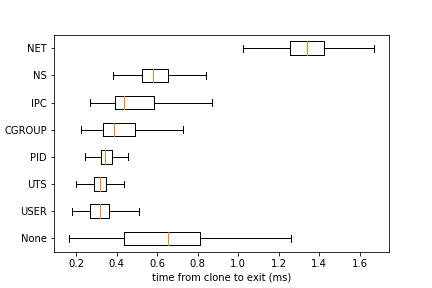
\includegraphics[width=0.7\textwidth]{graphs/clone_individual_namespaces.png}

    \caption{Performance of making the \texttt{clone(2)} system call with varying namespace creation flags. The test is run in a tight compiled C loop with high precision timings taken before and after each new process is cloned and waited for. \texttt{clone(2)} presents very noisy results on a system with background activity.}
    \label{fig:namespace-times}
\end{figure}

As void processes must create multiple namespaces to effectively isolate processes, creating multiple namespaces is shown in Figure \ref{fig:namespace-stacked-times}. Here the divide between the three slowest namespaces in Figure \ref{fig:namespace-times} is exaggerated, showing a significant divide between the quick four namespaces and the slow final three.

\begin{figure}
    \centering
    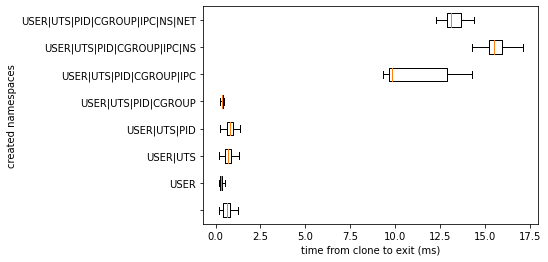
\includegraphics[width=0.8\textwidth]{graphs/clone_stacked_namespaces.png}

    \caption{Performance of making the \texttt{clone(2)} system call with increasing amounts of namespace creation flags. The effects of Figure \ref{fig:namespace-times} are amplified when creating multiple namespaces in a single call this frequently. There is a clear divide between the time taken for user, pid, uts, and cgroup namespaces and ipc, ns and net namespaces.}
    \label{fig:namespace-stacked-times}
\end{figure}

\section{Summary}

In this chapter I discussed the 8 namespaces available in Linux 5.15: what each namespace protects against, how to completely empty each created namespace, and the constraints in doing so. For cgroup and mount namespaces, alternative designs that increase the usability of the namespaces were discussed.

Emptying namespaces has been motivated by protection from vulnerabilities. Facilities to re-expose some of the system must now be introduced to build useful applications. The methods for reintroducing parts of the system are given in Chapter \ref{chap:filling-the-void}, before demonstrating how to build applications in Chapter \ref{chap:building-apps}.


\chapter{Filling the Void}
\label{chap:filling-the-void}

Now that a completely empty set of namespaces are available for a void process, the ability to reinsert specific privileges must be added to support non-trivial applications. This is achieved using a mixture of file-descriptor capabilities (§\ref{sec:priv-sep-ownership}) and adding elements to the empty namespaces (§\ref{sec:priv-sep-perspective}). Capabilities allow for very explicit privilege passing where suitable, while adding elements to namespaces supports more of Linux's modern features.

\section{Mount namespace}
\label{sec:filling-mount}

There are two options to provide access to files and directories in the void. For a single file, an opened file descriptor can be offered. Consider the TLS broker of a TLS server with a persistent certificate and keyfile. Only these files are required to correctly run the application - no view of a filesystem is necessary. Providing an already opened file descriptor gives the process a capability to those files while requiring no concept of a filesystem, allowing that to remain a complete void. This is possible because of the semantics of file descriptor passing across namespaces - the file descriptor remains a capability, regardless of moving into a namespace without the file.

Alternatively, files and directories can be mounted in the void process's namespace. This supports three things which the capabilities do not: directories, dynamic linking, and existing applications. Firstly, the existing \texttt{openat(2)} and resultant directory file descriptors are not suitable as capabilities - they only retain the path of their directory internally. This means that a process with a directory file descriptor in another namespace cannot use it to access files outside of the namespace, removing all utility as capabilities in the void. Secondly, dynamic linking is best served by binding files, as these read only copies and the trusted binaries ensure that only the required libraries can be linked against. Finally, support for individual required files can be added by using file descriptors, but many applications will not trivially support it. Binding files allows for some backwards compatibility with applications that are more difficult to adapt.

\section{Network namespace}
\label{sec:filling-net}

Reintroducing networking to a void process follows a similar capability-based paradigm to reintroducing files. Rather than providing the full Linux networking subsystem to a void process, it is instead handed a file descriptor that already has the requisite networking permissions. A capability for an listening networking socket can be requested statically in the application's specification. This socket remains open and allows the application to continuously accept requests, generating the appropriate socket for each request within the application itself. These request capabilities can be dealt with in the same void process or handed back to the shim to be distributed to another void process.

Outbound networking is more difficult to re-add to a void process than inbound networking. Containerisation solutions such as Docker use NAT with bridged adapters by default. That is, the container is provided an internal IP address that allows access to all networks via the host. Virtual machine solutions take a similar approach, creating bridged Ethernet adapters on the outside network or on a private NAT. Each of these approaches give the container/machine the appearance of unbounded outbound access, relying on firewalls to limit this afterwards. This does not fit well with the ethos of creating a void process - minimum privilege by default. An ideal solution would provide precise network access to the void, rather than adding all access and restricting it in post. This is achieved with inbound sockets by providing the precise and already connected socket to an otherwise empty network namespace, which does not support creating exposed inbound sockets of its own.

Consideration is given to providing outbound access with statically created and passed sockets, the same as inbound access - a socket to a database could be specified statically in the specification. The downside of this approach is that the socket lifecycle is still handled by the kernel. While this could work well with UDP sockets, TCP sockets can fail because the remote was closed or a break in the path caused a timeout to be hit.

Given that statically giving sockets is infeasible and adding a firewall does not fit well with creating a void, I sought an alternative API. \texttt{pledge(2)} is a system call from OpenBSD which restricts future system calls to an approved set \citep{the_openbsd_foundation_pledge2_2022}. This seems like a good fit, though operating outside of the operating system makes the implementation very different. Acceptable sockets are specified in the application specification, then an interaction socket is provided to request various pre-approved sockets from the shim. This allows limited access to the host network, approved or denied at request time instead of by a firewall. That is, access to a precisely configured socket can be injected to the void, with a capability to request such sockets and a capability given for each socket requested.

\section{User namespace}
\label{sec:filling-user}

Filling a user namespace is a slightly odd concept compared to the namespaces already discussed in this section. A user namespace comes with no implicit mapping of users whatsoever (§\ref{sec:voiding-user}). To enable applications to be run with bounded authority, a single mapping is added by the void orchestrator of \texttt{root} in the child user namespace to the launching UID in the parent namespace. This means that the user with highest privilege in the container, \texttt{root}, will be limited to the access of the launching user. The behaviour of mapping \texttt{root} to the calling user is shown with the \texttt{unshare(1)} command in Listing \ref{lst:mapped-root-directory}, where a directory owned by the calling user, \texttt{alice}, appears to be owned by \texttt{root} in the new namespace. A file owned by \texttt{root} in the parent namespace appears to be owned by \texttt{nobody} in the child namespace, as no mapping exists for that file's user.

\begin{listing}
\begin{minted}{shell-session}
£ ls -ld repos owned_by_root
-rw-r--r-- 1 root  root     0 May  7 22:13 owned_by_root
drwxrwxr-x 7 alice alice 4096 Feb 27 17:52 repos

£ unshare -U --map-root

# ls -ld repos owned_by_root
-rw-r--r-- 1 nobody nogroup    0 May  7 22:13 owned_by_root
drwxrwxr-x 7 root root 4096 Feb 27 17:52 repos
\end{minted}

\caption{A directory listing before and after entering a user namespace with mapped root demonstrates filesystem objects owned by the mapped (calling) user shown as being owned by root and any other filesystem objects shown as being owned by nobody.}
\label{lst:mapped-root-directory}
\end{listing}

The way user namespaces are currently used creates a binary system: either a file appears as owned by \texttt{root} if owned by the calling user, or appears as owned by \texttt{nobody} if not. One questions whether more users could be mapped in, but this presents additional difficulties. Firstly, \texttt{setgroups(2)} system call must be denied to achieve correct behaviour in the child namespace. This is because the \texttt{root} user in the child namespace has full capabilities, which include \texttt{CAP\_SETGID}. This means that the user in the namespace can drop their groups, potentially allowing access to materials which the creating user did not (consider a file with permissions \texttt{0707}). This limits the utility of switching user in the child namespace, as the groups must remain the same. Secondly, mapping to users and groups other than oneself requires \texttt{CAP\_SETUID} or \texttt{CAP\_SETGID} in the parent namespace. Avoiding this is well advised to reduce the ambient authority of the shim.

Voiding the user namespace initially provides the ability to create other namespaces with ambient authority, and hides the details of the void process's ambient permissions from inside. Although this creates a binary system of users which may at first seem limiting, applying the context of void processes demonstrates that it is not. Linux itself may utilise users, groups and capabilities for process limits, but void processes only provide minimum privilege by default. That is, if a process should not have access to a file owned by the same user, it is simply not made available. Running only as \texttt{root} within the void process is therefore not a problem - multiple users is a feature of Linux which doesn't assist void processes in providing minimum privilege, so is absent.

\section{Remaining namespaces}

\subsection{UTS namespace}
\label{sec:filling-uts}

UTS namespaces are easily voided by setting the two controlled strings to a static string. However, if one wishes for them to hold specific values, they can be set in one of two ways: either calling \texttt{sethostname(2)} or \texttt{setdomainname(2)} from within the void process, or by providing static values within the void process's specification.

\subsection{IPC namespace}
\label{sec:filling-ipc}

Filling IPC namespaces is also not possible in this context, as IPC namespaces are created empty (§\ref{sec:voiding-ipc}). IPC objects exist in one and only one IPC namespace, due to sharing what they expect to be a global namespace of keys. This means that existing IPC objects cannot be mapped into the void process's namespace. However, the process within the IPC namespace can use IPC objects, for example between threads. This is potentially inadvisable, because different void processes would provide stronger isolation than IPC within a single void process. Alternative IPC methods are available which use the filesystem namespace and are better shared between void processes.

\subsection{PID namespace}
\label{sec:filling-pid}

A created PID namespace exists by itself, with no concept of mapping in PIDs from the parent namespace. The first process created in the namespace becomes PID 1, and after that other processes can be spawned from within. As such there is no need to fill PID namespaces, instead applications can be restructured to not expect seeing other process's IDs.

\subsection{Control group namespace}
\label{sec:filling-cgroup}

cgroup namespaces present some very interesting behaviour in this regard. What appears to be the root in the new cgroup namespace is in fact a subtree of the hierarchy in the parent. This again provides a quite strange concept of filling - elements of the tree cannot be cloned to appear in two places, by design. To provide fuller interaction with the cgroups system, one can instead bind whichever subtree they wish to act on from the parent mount namespace to the child mount namespace. This provides the control of any section of the cgroups subtree seen fit, and is unaffected by the cgroups namespace of the child. That is, the cgroups namespace is used only to provide a void, and the mount namespace can be used to operate on cgroups.

\section{System design}
\label{sec:system-design}

At this point in the thesis the theory of creating a void process (§\ref{chap:entering-the-void}) and the theory of filling a void with enough privilege to do useful work have been laid out. Now I present some more detail on the system that combines these together in a useful aid to privilege separation.

The central contribution of void processes is the void orchestrator, a shim that uses an application binary and a textual specification to set up the multiple processes required for privilege separation. The specification describes a series of entrypoints, each of which contain three things: a trigger to create the process, a list of arguments, and extra elements for the environment. Example specifications are included in Chapter \ref{chap:building-apps}.

There are two types of entrypoints: those spawned statically at startup, and those spawned dynamically when triggered by an event. This event, as shown in the TLS server example (§\ref{sec:building-tls}), is most commonly sending one or more file descriptors from a different void process. File descriptors are the primary method of communication as they are not impacted by namespaces in any way - performance or isolation.

When a void process is spawned, the void orchestrator uses the specification to pass the pre-specified privilege into the void. A concept of spawners is also provided, which allows a void process to trigger the creation of another void process. Spawners are an additional process, existing in a void, which create further voids on demand. This allows for separation of privilege by handing work off to a differently privileged void when needed.

The void orchestrator handles the management of the void processes which make up an application, reducing the burden on the application programmer. A central knowledge bank for preparing a void serves as a single point to upgrade when new ambient authority is added and needs to be removed.

\section{Summary}

Included in the goal of minimising privilege is providing new APIs to support this. A mixed solution of capabilities, capability creating capabilities, and file system bind mounts is used to re-add privilege where necessary. Interface thinning is used to ban APIs which do not well suit the model. Now that void processes with useful privilege can be created, and software exists to orchestrate applications consisting of void processes, Chapter \ref{chap:building-apps} presents two example applications which utilise void processes for privilege separation.


\chapter{Building Applications}
\label{chap:building-apps}

This section discusses the process of creating applications which utilise void processes. An application which requires only basic privilege is demonstrated (§\ref{sec:building-fib}), showing how to put together a simple application that takes advantage of void processes to start with minimum privilege. We conclude with a basic HTTP file server with TLS support, designed and built from the ground up for void processes (§\ref{sec:building-tls}).

\section{Fibonacci}
\label{sec:building-fib}

To begin displaying the power of the void orchestrator system we will develop an application that requires very modest privilege. The application and its fixed output are shown, unmodified, in Listing \ref{lst:fibonacci-application}. It is written in Rust, my language of choice, but there is no such requirement - an equivalent program would look very similar in C. The limited code of this example makes the privilege requirements exceptionally clear. Computing \texttt{fib} requires no privilege at all, operating purely on numbers on the stack. Once the values are computed they are printed using the \texttt{println!} macro, which prints to stdout. Therefore the only privilege this application requires at runtime is access to stdout.

\begin{listing}
\begin{minted}{rust}
fn main() {
    println!("fib(1) = {}", fib(1));
    println!("fib(7) = {}", fib(7));
    println!("fib(19) = {}", fib(19));
}

fn fib(i: u64) -> u64 {
    let (mut a, mut b) = (0, 1);
    for _ in 0..i {
        (a, b) = (b, a + b);
    }
    a
}
\end{minted}
\begin{minted}[frame=bottomline]{shell-session}
fib(1) = 1
fib(7) = 13
fib(19) = 4181
\end{minted}

\caption{A basic Fibonacci application. The application computes elements of the Fibonacci sequence on static indices and does not process any user input.}
\label{lst:fibonacci-application}
\end{listing}

To run this application as a void process we require a specification (§\ref{sec:system-design}) to detail how the processes of the application should be set up. The specification for the Fibonacci application is given in Listing \ref{lst:fibonacci-application-spec}. When specifying an entrypoint for an application every privilege needed must be specified explicitly. In this case, as discussed, the application only requires special access to stdout. This is specified in the environment section of the entrypoint. We also see in the specification a variety of libraries made available, required for the application to successfully dynamically link. This information is decidable from the binary, but implementing that is left for future work (§\ref{sec:future-work-dynamic-linking}). We also see that no arguments are specified, although they are a part of the specification. No specified arguments defaults to no arguments, as the void orchestrator minimises privilege by default. The application void process therefore receives no arguments - including \texttt{arg0} as the binary name.

\begin{listing}
\begin{minted}{json}
{"entrypoints": { "fib": { "environment": [
    "Stdout",
    {
        "Filesystem": {
            "host_path": "/lib/x86_64-linux-gnu/libgcc_s.so.1",
            "environment_path": "/lib/libgcc_s.so.1"
        }
    },
    {
        "Filesystem": {
            "host_path": "/lib/x86_64-linux-gnu/libc.so.6",
            "environment_path": "/lib/libc.so.6"
        }
    },
    {
        "Filesystem": {
            "host_path": "/lib64/ld-linux-x86-64.so.2",
            "environment_path": "/lib64/ld-linux-x86-64.so.2"
        }
    }
]}}}
\end{minted}

\caption{The specification for the void orchestrator to run the application shown in Listing \ref{lst:fibonacci-application}. A single entrypoint is provided with a minimal environment, including only the content to dynamically link the binary and standard output.}
\label{lst:fibonacci-application-spec}
\end{listing}

More of the advanced features of the system will be shown in the second example, but this is enough to get a basic application up and running. We can see that the Rust application looks exactly like it would without the shim. The application is also fully deprivileged. Of course, for an application as small as this example, we can verify by hand that the program has no foul effects. We can imagine a trivial extension that would make this program more dangerous: using a user argument (a privilege the program does not currently have) to take a value on which to execute fib. One way this user input could cause damage is with flawed usage of a logging library. The recent widespread example is Log4j2 with CVE-2021-44228, enabling an attacker with string control to execute arbitrary code from the Internet. A void process with privilege of only arguments and stdout would protect well against this vulnerability, as not only is there no Internet access to pull remote code, but there is nothing to take advantage of in the process even if remote code execution is gained.

\subsection{Performance}
\label{sec:fib-performance}

In Section \ref{sec:void-creation-costs} testing showed that creating all of the namespaces needed for a void can have extremely high overhead compared to creating a simple new process. Now that a basic application exists to evaluate this on, the latency of the final shim executing an application can be tested.

Figure \ref{fig:fib-launch-times} shows the difference in spawning an application directly and spawning it with the shim (the Fibonacci application is compatible with both). A C application with a tight for loop is compiled, which calls \texttt{vfork(2)} followed by \texttt{wait(2)}, again using high precision \texttt{CLOCK\_MONOTONIC} timings. The child process calls \texttt{execv(2)} immediately, in the direct case with the Fibonacci binary itself, and in the shim case with the shim with the Fibonacci specification and binary as arguments.

\begin{figure}
    \centering
    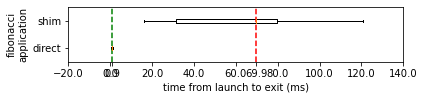
\includegraphics[width=0.6\textwidth]{graphs/fib_startup.png}

    \caption{A box plot comparing the performance of the Fibonacci example (§\ref{sec:building-fib} under the shim and called directly. The median time to run under the shim is approximately 800\% the time without. The inter-quartile range and range of results is also much larger.}
    \label{fig:fib-launch-times}
\end{figure}

The results demonstrate both significantly higher median latency and significantly higher variance in the results. The machine is the same as that mentioned in Section \ref{sec:void-creation-costs}. Although my virtual machine was not particularly busy at the time of testing, it appeared that the underlying host was, affecting times due to virtual machine context switching within the hypervisor. The underlying trend of a significant overhead remained throughout testing. This thesis focused on user-space, but future work in kernel-space should be able to reduce this overhead (§\ref{sec:future-work-kernel-api}).

\section{TLS server}
\label{sec:building-tls}

Rather than presenting the complete applications as shown in the previous two sections, the TLS server presents instead a case study on designing applications from the ground up to run as void processes. The thought process behind data flow design and taking advantage of the more advanced void orchestrator features is given. This results in the process separation presented in Figure \ref{fig:tls-server-processes}. First we must accept TCP requests from the end user (§\ref{sec:building-tls-tcp-listener}). Then, to be able to check that all is working so far, we respond to these requests (§\ref{sec:building-tls-http-handler}). Finally, we add an encryption layer using TLS (\ref{sec:building-tls-tls-handler}). This results in a functional TLS file server with strong privilege separation, with each stage having exactly the privilege that it requires.

\begin{figure}
    \centering
    \includestandalone[width=0.8\textwidth]{diagrams/tls-server-processes}

    \caption{The final process design for a TLS server running under the void orchestrator. The figure is split into processes running void orchestrator code and processes running user code. Arrows represent a passing of privilege from one process to another.}
    \label{fig:tls-server-processes}
\end{figure}

\subsection{TCP listener}
\label{sec:building-tls-tcp-listener}

The special privilege required by a process which accepts TCP connections is a listening TCP socket. As discussed in Section \ref{sec:filling-net}, TCP listening sockets are handed already bound to void processes. This enables a capability model for network access, otherwise restricting inbound and outbound networking entirely. The specification for this listener is given in Listing \ref{lst:tls-tcp-listener-spec}, where the TCP listener is requested as an argument already bound. No other permissions are required to accept connections from a TCP listener. Although the code at each stage is omitted for brevity, the resulting program has to parse the argument back into an integer and then a \texttt{TcpStream} before looping to receive incoming connections. When building and debugging software it is often useful to have access to the \texttt{stdout} or \texttt{stderr} streams, even though they won't be utilised in production. The void orchestrator provides useful \texttt{--stdout} and \texttt{--stderr} flags to temporarily privilege an application for debugging without modifying its specification. Having a process that can accept TCP streams but no nothing else is of little use, except for a simple hello world example or echo example. We move on to developing the HTTP handler to see useful output from the application.

\begin{listing}
\begin{minted}{json}
{"entrypoints": { "tcp_listener": {
	"args": [
		{ "TcpListener": { "addr": "0.0.0.0:8443" } }
	]
}}}
\end{minted}

\caption{The void orchestrator specification for the TCP listener endpoint of the TLS application. The privilege to use a TCP listener is requested as an argument. Dynamic linking binds are omitted for brevity.}
\label{lst:tls-tcp-listener-spec}
\end{listing}

\subsection{HTTP handler}
\label{sec:building-tls-http-handler}

When attempting to add the HTTP handler, we immediately require more privilege. As this is intended to be a file server, we need some files. Although it would be easy to add files to the existing entrypoint, the principle of least privilege is highly encouraged when developing a void process. One should always ask whether an entrypoint needs a new privilege that they are about to add to it, or whether they would be better served with a new entrypoint.

In this case, we are going to add a new entrypoint for two reasons: multiprocessing and privilege separation. This allows the TCP listener entrypoint to continue in a tight loop, accepting requests very quickly and fanning them out to new processes. These new processes have only their required privileges: the files they wish to serve, and the \texttt{TcpStream} to serve them over. We take advantage here of another feature of the void orchestrator, file socket based triggers. These allow a statically defined socket to be setup which the void orchestrator will listen on and create new void processes on demand. Further, this ensures isolation between requests, meaning that a single failed request which causes a process to fail will not affect any others, and a compromised process can't leak information about any other requests.

The HTTP handler entrypoint is added to the specification in Listing \ref{lst:tls-http-handler-spec}. As well as adding a single extra argument to trigger the HTTP handler, we must also add an entrypoint argument to differentiate between the two entrypoints. Much like the usage of \texttt{arg0} for symlinked binaries, we utilise \texttt{arg0} to find which intended use of the binary is being called (Listing \ref{lst:tls-main-function}). Having looked at this specification, we can imagine what the code for each section would look like. Tight privilege bounds act somewhat like type signatures in dictating the behaviour of an application. Future work involves taking more advantage of this link between the two (§\ref{sec:future-work-macros}).

\begin{listing}
\begin{minted}{json}
{"entrypoints": {
    "tcp_listener": {
        "args": [
            "Entrypoint",
            { "FileSocket": { "Tx": "http" } },
            { "TcpListener": { "addr": "0.0.0.0:8443" } }
        ]
    },
    "http_handler": {
        "trigger": { "FileSocket": "http" },
        "args": [ "Entrypoint", "Trigger" ],
        "environment": [{ "Filesystem": {
            "host_path": "/var/www/html",
            "environment_path": "/var/www/html"
        }}]
    }
}}
\end{minted}

\caption{The void orchestrator specification for the TCP listener endpoint and HTTP handler endpoint of the TLS application. This extends on Listing \ref{lst:tls-tcp-listener-spec} by adding the HTTP handler endpoint. A new File Socket is used to link the two entrypoints together. Dynamic linking binds are omitted for brevity.}
\label{lst:tls-http-handler-spec}
\end{listing}

\begin{listing}
\begin{minted}{rust}
fn main() {
    match std::env::args().next() {
        Some(s) => match s.as_str() {
            "connection_listener" => connection_listener_entrypoint(),
            "http_handler" => http_handler_entrypoint(),
            _ => unimplemented!(),
        },
        None => unimplemented!(),
    }
}
\end{minted}

\caption{The main function for the TLS server. This matches on the entrypoint arg0 to determine which entrypoint the application has been run for.}
\label{lst:tls-main-function}
\end{listing}

\subsection{TLS handler}
\label{sec:building-tls-tls-handler}

The final stage is to add the TLS handling into the mix. Once again we have the choice of whether to add this to an existing entrypoint or create a new one. This decision is very similar to HTTP handling, but perhaps more important. Rather than adding the \texttt{www} directory that we intend to serve publicly anyway, we are entrusting a process with the private keys of the TLS certificate, allowing anyone who takes over the process to impersonate us. This is again an excellent time for more privilege separation, so the TLS handling will be added as an additional entrypoint.

The resulting specification is given in Listing \ref{lst:tls-spec}. The TLS handler is added in a very similar manner to the previous HTTP handler. It is triggered by a file socket, but this time receives another file socket to trigger the next stage. It receives file descriptor capabilities to each the certificate and private key files, along with the TCP stream. This process receives nothing but highly restricted capabilities, ensuring that there is very little attack surface for compromise.

\begin{listing}
\begin{minted}{json}
{"entrypoints": {
    "connection_listener": {
        "args": [
            "Entrypoint",
            { "FileSocket": { "Tx": "tls" } },
            { "TcpListener": { "addr": "0.0.0.0:8443" } }
        ]
    },
    "tls_handler": {
        "trigger": { "FileSocket": "tls" },
        "args": [
            "Entrypoint",
            { "FileSocket": { "Tx": "http" } },
            { "File": "/etc/ssl/certs/example.com.pem" },
            { "File": "/etc/ssl/private/example.com.key" },
            "Trigger"
        ]
    },
    "http_handler": {
        "trigger": { "FileSocket": "http" },
        "args": [ "Entrypoint", "Trigger" ],
        "environment": [{ "Filesystem": {
            "host_path": "/var/www/html",
            "environment_path": "/var/www/html"
        }}]
    }
}}
\end{minted}

\caption{The void orchestrator specification for the final TLS application. This extends on Listing \ref{lst:tls-tcp-listener-spec} by adding the HTTP handler endpoint. A new File Socket is used to link the two entrypoints together. Dynamic linking binds are omitted for brevity.}
\label{lst:tls-spec}
\end{listing}

We now have a full specification for a TLS server. In this section I have focused entirely on building up the specification and not the code behind it. There are two reasons for this: the code has a lot of boilerplate argument processing, and a variety of code implementations are available. The boilerplate argument processing could be addressed with future work using features like proc macros in Rust which dynamically generate code based on input (§\ref{sec:future-work-macros}). As for varying implementations, I chose to use the static library \texttt{rustls} to implement my TLS server. There are many excellent alternatives, such as OpenSSL and LibreSSL, which would work just as well though with different APIs. For HTTP I use a Rust crate for request parsing, before responding only to \texttt{GET} requests. The isolation from sensitive material adds a degree of freedom to request handling, as there is so little which can go wrong. The implementation therefore matters very little in this analysis, but is made available at \ifsubmission\url{file:///SUBMITTED_SRC/void-orchestrator/examples/tls/}\else\url{https://github.com/JakeHillion/void-orchestrator/tree/main/examples/tls/}\fi. Instead the focus is on composability and privilege separation, showing the flexibility of the system.

\subsection{Performance}
\label{sec:tls-performance}

The performance of the TLS server provides a much more nuanced view than the performance of the trivial Fibonacci example (§\ref{sec:fib-performance}). I evaluated my void process solution against \texttt{apache2}, a highly tuned HTTP server. Both used the same self-signed TLS certificate and were benchmarked with \texttt{ab}, the Apache HTTP server benchmarking tool. The machine setup remains the same as in Section \ref{sec:void-creation-costs}. \texttt{apache2} runs the standard Ubuntu 22.04 LTS config with the TLS module enabled.

Figure \ref{fig:tls-performance} shows the number of requests per second achieved over a ten second testing period, where \texttt{ab} created 100 concurrent connections and was allowed unlimited total requests. The graph plots the median result and the interquartile range. Figure \ref{fig:tls-relative-performance} shows the same data, but this time divided by the median result of the apache server's benchmark, allowing easier analysis of the relative performance of the two solutions.

\begin{figure}
    \centering
    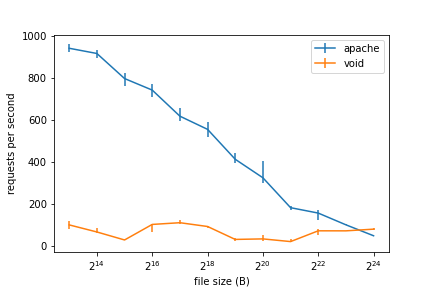
\includegraphics[width=0.8\textwidth]{graphs/tls_performance.png}

    \caption{\texttt{a2bench} requests per second results over 10 seconds with 100 simultaneous requests on varying response sizes. As the response size increases, the gap between the \texttt{apache2} TLS web server and the void process TLS web server decreases.}
    \label{fig:tls-performance}
\end{figure}

\begin{figure}
    \centering
    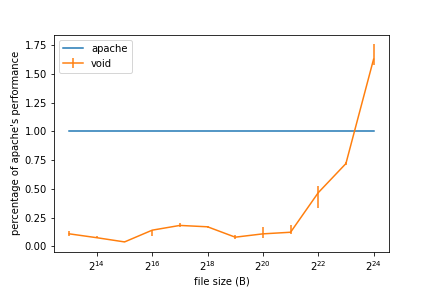
\includegraphics[width=0.8\textwidth]{graphs/tls_relative_performance.png}

    \caption{\texttt{a2bench} requests per second results over 10 seconds with 100 simultaneous requests on varying response sizes. As the response size increases, the gap between the \texttt{apache2} TLS web server and the void process TLS web server decreases. Results are scaled to the \texttt{apache2} medians, and \texttt{apache2} is shown with no error as it is always 100\% of itself.}
    \label{fig:tls-relative-performance}
\end{figure}

The trend of the data is that the void process solution handles large request sizes better, while \texttt{apache2} handles small request sizes significantly better. This relates to the high cost of process creation (§\ref{sec:void-creation-costs},§\ref{sec:fib-performance}) associated with void processes, given that two processes need be created for each request (a \texttt{tls\_handler} and a \texttt{http\_handler}). However, combined with large response processes (meaning long lived processes) and high concurrency, the void process server eventually outperforms \texttt{apache2}. This highlights the effectiveness of using ordinary file descriptors as performance is maintained, even with maximum privilege separation.

\section{Summary}

I've demonstrated how void processes can both run a standard process with no privilege requirements and define a structure for a new application. Explicit definitions of privilege can make it very clear to the programmer where privilege boundaries are, leading to effective privilege separation. The performance changes caused by these designs have been evaluated, where the use of standard file descriptors as capabilities shows that utilising the void orchestrator can achieve acceptable performance with minimal programming effort.


\chapter{Conclusions}
\label{chap:conclusions}

The system built in this project enables running applications with minimal privilege in a Linux environment in a novel way. Performance is shown to be comparable, and demonstrates where the existing kernel setup provides inadequate performance for such applications. Design choices in the user-space kernel APIs for namespaces are discussed and contextualised, with suggestions offered for alternate designs.

Void processes offer a new paradigm for application development which prioritises minimal privilege. Applications often need to be completely rewritten in order to take advantage of improved isolation, rather than being limited by backwards compatibility guarantees. The system is designed to support effective static analysis on applications, though this is not implemented at this stage. I present in this work that privilege through explicit choices is a simpler paradigm for programmers than fighting against the moving target of Linux ambient privilege.

Finally, void processes provide a seamless experience without making kernel-space changes, allowing for ease of deployment. It runs on the Linux kernel, a production kernel with widespread usage. Although the current kernel structure limits the performance of the work with the namespace creation bottleneck, the feasibility of namespaces for process isolation is effectively demonstrated in a system that encourages application writers to develop with privilege separation as a first principle.

\section{Future Work}
\label{sec:future-work}

\subsection{Kernel API improvements}
\label{sec:future-work-kernel-api}

The primary future work to increase the utility of void processes is better performance when creating empty namespaces. Sections \ref{sec:void-creation-costs} and \ref{sec:fib-performance} showed that the startup hit when creating the namespaces for a void is very high. This shows a limitation of the APIs, as creating a namespace that has no relation to a parent should involve a small amount of work. Secondly, an API similar to network namespaces adding paired interfaces between namespaces should be added for binding in mount namespaces, allowing mount namespaces to be created completely empty. This would also benefit containers which by default have no connection to the parent namespace, but need to mount in their own root filesystem.

\subsection{Dynamic linking}
\label{sec:future-work-dynamic-linking}

Dynamic linking works correctly under the shim, however, it currently requires a high level of manual and static input. If one assumes trust of the binary as well as the specification, it is feasible to add a pre-spawning phase which appends read-only libraries to the specification for each spawned process automatically before creating appropriate voids. This would allow anything which can link correctly on the host system to link correctly in void processes with no additional effort.

\subsection{Building specifications from code}
\label{sec:future-work-macros}

Much of the information given in the specification and the code is shared. For example, the specification may list the arguments and also imply their type. This means that a function signature for an entrypoint implies almost all of the specification of an entrypoint, which would allow effective code generation with some supplementary information. This would remove many of the boilerplate argument processing lines from the examples and increase the usability of the system. Combining this with the dynamic linking work (§\ref{sec:future-work-dynamic-linking}) would remove a huge amount of the manual effort in creating the specification, making the system more user friendly.

\label{lastcontentpage} % end page count here
%TC:ignore              % end word count here

\bibliographystyle{PhDbiblio-url} 
\bibliography{references}

\appendix

\label{lastpage}
%TC:endignore
\end{document}
